\documentclass[xcolor=pdftex,dvipsnames,table,mathserif,aspectratio=169]{beamer}
\usetheme{metropolis}

%\usetheme{Darmstadt}
%\usepackage{times}
%\usefonttheme{structurebold}

\usepackage[english]{babel}
%\usepackage[table]{xcolor}
\usepackage{pgf,pgfarrows,pgfnodes,pgfautomata,pgfheaps}
\usepackage{amsmath,amssymb,setspace,centernot}
\usepackage[latin1]{inputenc}
\usepackage[T1]{fontenc}
\usepackage{relsize}
\usepackage{stmaryrd}
\usepackage{pdfpages}
\usepackage{booktabs}
\usepackage[absolute,overlay]{textpos} 


\newenvironment{reference}[2]{% 
  \begin{textblock*}{\textwidth}(#1,#2) 
      \footnotesize\it\bgroup\color{red!50!black}}{\egroup\end{textblock*}} 

\DeclareMathSizes{10}{10}{6}{6} 
\AtBeginSection[]{
  \begin{frame}
  \vfill
  \centering
  \begin{beamercolorbox}[sep=8pt,center,shadow=true,rounded=true]{title}
    \usebeamerfont{title}\insertsectionhead\par%
  \end{beamercolorbox}
  \vfill
  \end{frame}
}
\begin{document}
\title{Antitrust}
\author{Chris Conlon}
\institute{Grad IO}
\date{\today}

\frame{\titlepage}

\begin{frame}
\frametitle{What is Antitrust?}
 \begin{itemize}
\item Current Debate: should we maximize \alert{efficiency/social surplus} or should we focus on \alert{consumer surplus}.
\begin{itemize}
\item US antitrust law focuses primarily on harm to consumers.
\item EC tends to also worry about harm to competing firms.
 \end{itemize}
 \item We know about DWL from market power from undergrad economics. However, without profits, why would firms innovate or perform R\&D?
 \begin{itemize}
\item Law understands this and awards temporarily monopolies via patents.
 \end{itemize}
\item Today, I am going to focus mostly on \alert{horizontal mergers} among competitors.
\begin{itemize}
\item Most of this is known as \alert{unilateral effects} (which is a terrible name).
\item Also worry about \alert{coordinated effects} which mean the nature of equilibrium changes.
 \end{itemize}
 \end{itemize}
\end{frame}

\begin{frame}
\frametitle{Antitrust Legislation : Sherman Act (1890)}
 \begin{description}
\item [Section 1]``Every contract, combination in the form of trust or otherwise, or conspiracy, in restraint of trade or commerce among the several States, or with foreign nations, is declared to be illegal'' (Violation involves an \alert{agreement}).
\item [Section 2] ``Every person who shall monopolize, or attempt to monopolize, or combine or conspire with any other person or persons, to monopolize any part of the trade or commerce among the several States, or with foreign nations, shall be deemed guilty of a felony''.
 \end{description}
 Three \textit{per se} violations
 \begin{itemize}
 \item (1) price fixing (2) horizontal market division (3) refusals to deal.
 \item Other violations are \textit{rule of reason}.
 \end{itemize}
 
\end{frame}

\begin{frame}
\frametitle{Antitrust Legislation : Clayton Act (1914)}
 \begin{description}
\item [Section 2] Prohibits some forms of price discrimination, but only when it lessens competition.
\item [Section 3] Prohibits sales based on the condition that the buyer not buy from your competitor (includes tying and exclusive dealing), but only when effect may be to substantially lessen competition.
\item [Section 7] Prohibits mergers where the effect of such acquisition may be substantially to lessen competition, or tend to create a monopoly in any line of commerce.
\item [Section 8] Prevents a person from being a director of multiple competing firms.
 \end{description}
\end{frame}

\begin{frame}
\frametitle{Antitrust Legislation : Hart-Scott-Rodino Act (1976)}
 \begin{itemize}
\item Required pre-notification and registration of large mergers
\begin{itemize}
\item Transaction: \$78.2 million
\item Size of Person: \$156.3 M with target of \$15.6 M or total transaction of \$312.6M
\item These are ``inflation adjusted'' each year.
\end{itemize}
\item Initial review period is 30 days after which DOJ/FTC can request additional information or allow merger to proceed.
\item Second review usually involves detailed information about  price-cost margins, market shares, etc. (Usually more info available than to academic researchers).
\item Can request information company would reasonably have (customer surveys, etc.).
\item After second review can ask for \alert{injunctive relief} or \alert{remedies} which merging parties can oppose in court.
 \end{itemize}
\end{frame}

\begin{frame}{Wollman: AER: Insights: Stealth Consolidation}
Abrupt change to the transaction size was passed with other legislation, led to large change in newly exempted merger filings (for horizontal mergers).
\begin{center}
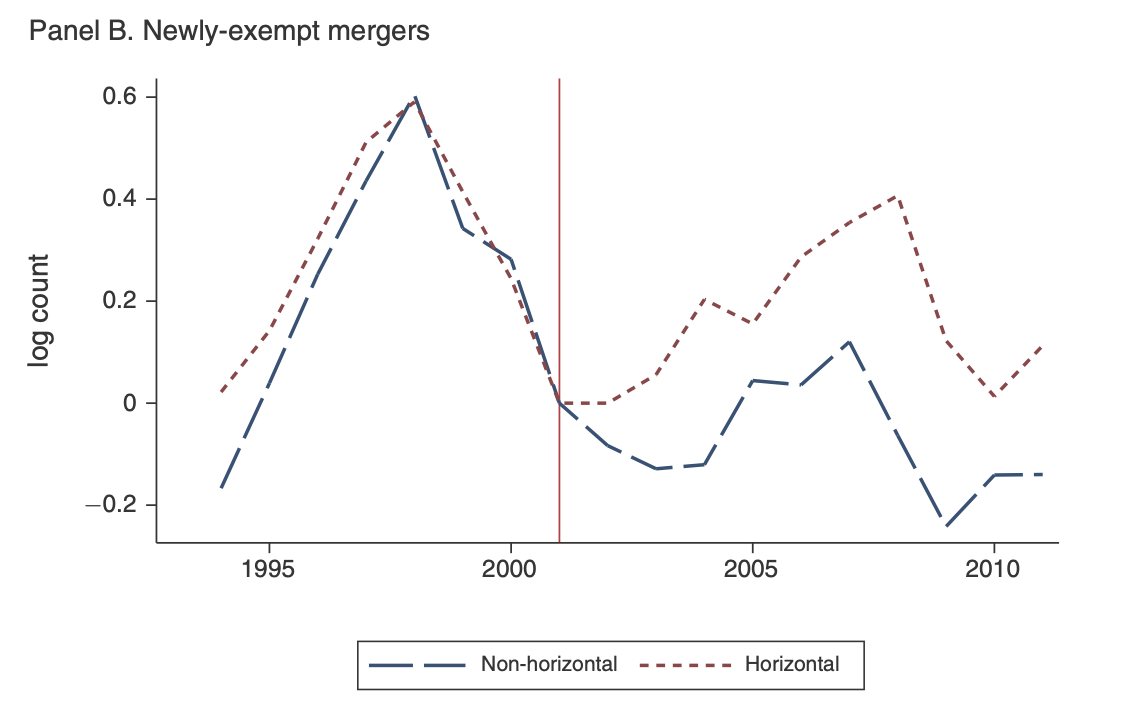
\includegraphics[height=0.8\textheight]{resources/wollman_consolidation.png}
\end{center}
\end{frame}

\begin{frame}
\frametitle{DOJ/FTC Horizontal Merger Guidelines}
 \begin{itemize}
\item DOJ/FTC describe markets as:
\begin{itemize}
\item Highly Concentrated: $HHI \geq 2500$.
\item Moderately Concentrated: $HHI \in [1500,2500]$. $\Delta HHI \geq 250$ merits scrutiny.
\item Un-Concentrated: $HHI \leq 1500$.
\end{itemize}
\item Also consider \alert{unilateral effects}/UPP and \alert{coordinated effects}.
\item Three steps:
\begin{enumerate}
\item Market Definition
\item Measure Concentration/Initial Screening
\item Merger Simulation
\end{enumerate}
 \end{itemize}
\end{frame}

\begin{frame}
\frametitle{Step 1: Market Definition}
SSNIP
 \begin{itemize}
\item Small but significant and non-transitory increase in price (SSNIP): smallest relevant market where a hypothetical monopolist could impose a 5\% price increase. (For at least one year).
\item Under linear demand this amounts to a price cost margin and an elasticity (sometimes the \alert{critical elasticity}).
 \end{itemize}
 Tricky Examples:
  \begin{itemize}
\item Whole Foods vs. Wild Oats
\item Cellophane Fallacy.
 \end{itemize}
\end{frame}

\begin{frame}
\frametitle{Step 2: Concentration/Screening}
 \begin{itemize}
\item After we define the relevant market, compute the relevant HHI or UPP.
\item There can be both geographic and product market issues in the relevant market.
\item Some markets may be highly concentrated and others may not be.
\item Can ask for \alert{divestitures} as part of a \alert{remedy} if there are a few problematic markets in an otherwise uncontroversial merger.
 \end{itemize}
\end{frame}


\begin{frame}
\frametitle{Step 3: Merger Simulation}
 \begin{itemize}
\item Simulate the price effects of the merger
\item Take into account likely cost synergies (sometimes there are none).
\item Estimate post-merger prices and welfare.
 \end{itemize}
 This is what we will talk about next.
\end{frame}













\end{document}